While CNNs can recognize objects well, they will often struggle to delineate them well. To solve this issue, Zheng et al. propose combining CNNs with conditional random fields (as in Eq. \ref{eq:costFunc}) working as a recurrent neural network (RNN) \cite{crfAsRNN}. 

\begin{figure}[h!]
\centering
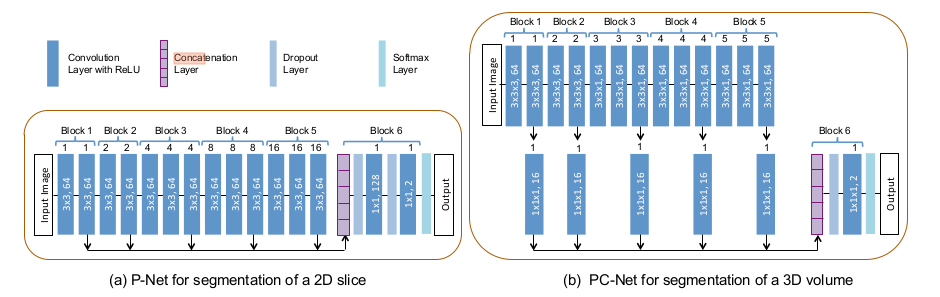
\includegraphics[scale=0.45]{pictures/P-Net}
\caption{The dilated convolution network for 2D (a) and 3D (b) segmentation used in DeepIGeoS and BIFSeg. The numbers in the boxes give the size of the weight matrix and number of output channels, and the number on top denotes the dilation parameter \cite{deepIGeoS}}
\label{fig:p-net}
\end{figure}

DeepIGeoS is a framework built by Wang et al. which is inspired by the work of Zheng et al. \cite{deepIGeoS}. DeepIGeoS has 2 CNNs, one to perform the initial segmentation (called P-Net), and a second to refine the segmentation according to user input (R-Net). Convolutional layers use dilated convolution in order to extract progressively larger features without reducing the resolution of the original image (see figure \ref{fig:p-net}). Both networks then have an RNN (Recurrent Neural Network) working as a CRF attached to the end of a CNN in order to improve the segmentation. Wang et al. slightly alter the RNNs such that the pairwise term is itself produced by a fully connected neural network. This pairwise network is pre-trained to produce a function like in Eq. \ref{eq:boundTerm}, but may change during training of the full network. 

Once P-Net and its CRF network have produced a first estimate, the user may mark on the image pixels which should be part of the object or the background, but have been mislabelled. Geodesic distance maps are then produced from this input, and these maps, alongside the original image and the segmentation map produced by P-Net and the CRF network are all combined by channel concatenation, and used as input to R-Net. The geodesic distance is the length of the shortest path between 2 pixels, where each pixel is connected by an edge which depends on intensity differences to its direct neighbours, usually with a function of the form
\begin{equation}
1 - e^{\frac{(I_1 - I_2)^2}{2 \sigma_{g}^{2}}} + l
\label{eq:geodesic}
\end{equation}
where $I_1$ and $I_2$ are the intensity values of the two pixels, $\sigma$ is some chosen parameter and $l$ is a minimum path length.
User interaction is simulated during the training of R-Net by randomly re-labeling mislabelled pixels. Wang et al. find that DeepIGeoS performs better segmentations than the FCN of Long et al. \cite{fcn}. 